\documentclass[NormeDiProgetto.tex]{subfiles}

\begin{document}
	
	\chapter{Processi organizzativi}
	
	\section{Comunicazione}
	In questa sezione vengono illustrate le norme che regolano la comunicazione sia tra i membri del gruppo 353 che con entità esterne, come i Committenti e i Proponenti.
	\subsection{Comunicazioni interne}
	Le comunicazioni interne al gruppo vengono effettuate tramite \Glossario{Slack}, un'applicazione di messaggistica multi piattaforma con funzionalità specifiche per gruppi di lavoro. La decisione di utilizzare questo strumento è stata supportata dalle funzionalità di integrazione di \Glossario{Bot} e di creazione di canali tematici, utili per poter classificare le conversazioni e permettere una comunicazione più efficace e mirata. 
	\\
	Inoltre è stato deciso di affiancare \Glossario{Skype} per effettuare video chiamate in caso di impossibilità di riunirsi personalmente. \'{E} stato scelto questo metodo poiché immediato e di facile utilizzo.
	\\
	All'interno di \Glossario{Slack} sono stati predisposti dei canali tematici, suddivisi per argomento in questo modo:
	\begin{itemize}
		\item \textbf{general}: Per discutere tutto ciò che riguarda l'organizzazione generale del progetto, la scelta degli strumenti di lavoro e per prendere decisioni in modo rapido. Inoltre qui vengono decisi gli argomenti principali da discutere nelle riunioni;
		\item \textbf{calendario\underline{ }meeting}: Il canale riservato nel quale un \Glossario{Bot} notifica giornalmente gli eventi facenti parte del calendario comune, come riunioni interne, eventi di formazione o riunioni esterne;
		\item \textbf{daily\underline{ }standup}: Il canale dedicato a un \Glossario{Bot} che giornalmente chiede ai partecipanti notizie sulle attività svolte nel giorno precedente e quelle che sono programmate per il giorno corrente. Inoltre viene chiesto se si sono verificati problemi nelle attività in corso, così da aiutare il gruppo a organizzarsi e a concentrare gli sforzi su particolari attività;
		\item \textbf{github\underline{ }notifications}: Il canale creato affinché un \Glossario{Bot} invii una notifica ogni qualvolta un membro del gruppo effettua un operazione su Github;
		\item \textbf{random}: Un canale generico, dove il gruppo discute liberamente di questioni non riguardanti il progetto e il suo sviluppo.
		
	\end{itemize}
	Sono stati creati anche dei canali appositi per gestire meglio la stesura dei documenti, nello specifico:
	\begin{itemize}
		\item \textbf{analisi\underline{ }requisiti}: Per commentare i casi d'uso e i requisiti necessari per la stesura del documento Analisi Dei Requisiti;
		\item \textbf{piano\underline{ }progetto}: Per confrontarsi sulla ripartizione dei ruoli e del monte ore a essi associato da includere nel Piano di Progetto;
		\item \textbf{piano\underline{ }qualifica}: Per discutere riguardo gli obiettivi e le strategie da applicare per garantire qualità e gestire verifica e validazione.
	\end{itemize}
	
	\subsection{Comunicazioni esterne}
	Questa sottosezione raccoglie le norme che regolano le comunicazioni con soggetti esterni al gruppo 353, i quali sono:
	\begin{itemize}
		\item La proponente \textbf{RedBabel} rappresentata da Alessandro Maccagnan e Milo Ertola, con i quali si intende stabilire un rapporto di collaborazione a fine di definire i requisiti che permetteranno la realizzazione del prodotto;
		\item \textbf{Prof. Tullio Vardanega} e \textbf{Prof. Riccardo Cardin}, ai quali verrà fornita la documentazione richiesta in ciascuna revisione di progetto, con i quali si intende dialogare con fine il miglioramento continuo.
	\end{itemize}
	\paragraph{Comunicazioni esterne scritte}
	Le comunicazioni esterne scritte vengono effettuate utilizzando l'indirizzo email del gruppo:
	\begin{center}
		\href {353swe@gmail.com}{353swe@gmail.com}
	\end{center}
	a cui ogni membro del gruppo ha accesso.\\
	Per comunicare con i Proponenti vengono utilizzati gli indirizzi email forniti durante la presentazione dei capitolati, rispettivamente 
	\begin{center}
		\href{alessandro@redbabel.com}{alessandro@redbabel.com} \\
		e\\
		\href{milo@redbabel.com}{milo@redbabel.com}
		
	\end{center}
	Inoltre è stato creato in \Glossario{Slack} un canale apposito per comunicare in maniera immediata con i proponenti, per accordarsi riguardo eventuali incontri e specifiche di progetto.\\
	Per comunicare con i Committenti si utilizza l'indirizzo di posta elettronica, utilizzando un oggetto specifico e conciso per descrivere il contenuto del messaggio. Ci si rivolge ai committenti dando loro del Voi o del Lei.
	
	\section{Riunioni}
	Questa sotto-sezione definisce le regole che normano le riunioni, interne o esterne, e il loro svolgimento.\\
	Durante lo svolgimento di ogni riunione, verrà nominato un segretario tra i membri del gruppo 353, il cui compito verterà nel far rispettare l'ordine del giorno, annotare gli argomenti discussi e redarre il Verbale di Riunione.
	\subsection{Verbale di riunione}
	Redigere il Verbale di Riunione è il compito del segretario, che dovrà essere strutturato secondo questo scheletro:
	\begin{itemize}
		\item \textbf{Verbale Esterno del DATA} che costituirà il frontespizio. Per DATA si intende il giorno in cui si è svolta la riunione;
		\item \textbf{Informazioni sulla riunione}: Questa sezione contiene:
		\begin{itemize}
			\item \textbf{Luogo e Data}: Ad esempio, Padova 05 Dicembre 2017;
			\item \textbf{Ora di inizio}: Nel formato ventiquattro ore, ad esempio 13:15;
			\item \textbf{Ora di fine}: Nel formato ventiquattro ore, ad esempio 15:30;
			\item \textbf{Partecipanti}: Elencati iniziando da Proponente/Committenti se la riunione è esterna, seguiti dai membri del gruppo partecipanti;
			\end{itemize}
			\item \textbf{Ordine del Giorno}: Indicato come elenco puntato degli argomenti da discutere;
			\item \textbf{Resoconto}: Contiene il riassunto redatto dal segretario secondo i punti dell'ordine del giorno, precisando se sono stati discussi e le loro relative discussioni.

	\end{itemize}
	\paragraph{Nomenclatura e Conservazione} I file relativi ai verbali dovranno essere nominati
	\begin{center}
		VER-DATA
	\end{center}
	ad esempio VER-2017-12-05, per permettere una facile organizzazione dei documenti.\\
	Essendo documenti ufficiali, devono essere redatti in \LaTeX e inclusi nella \Glossario{repository} omonima.
	
	\subsection{Riunioni interne}
	La partecipazione alle riunioni interne è permessa ai soli membri del gruppo 353.
	Il \textbf{Responsabile di Progetto} ha il compito di stilare l'ordine del giorno, fissare la data e inserirla nel calendario e approvare il verbale redatto dal Segretario.\\
	Di contro, i \textbf{partecipanti} devono presentarsi puntualmente alle riunioni, comunicare eventuali ritardi e partecipare attivamente alle discussioni.\\
	Affinché una riunione sia ritenuta valida, devono essere presenti almeno cinque membri del gruppo 353.
	\subsection{Riunioni esterne}
	Le riunioni esterne vedono coinvolti sia i membri del gruppo 353 che alcuni soggetti esterni.\\
	Principalmente le riunioni esterne vengono svolte in Torre Tullio Levi Civita, previa disponibilità dei locali.\\
	A causa della locazione europea dell'azienda proponente, le riunioni verranno effettuate tramite \Glossario{Skype}, per ovviare così al problema di distanza fisica.
	
	\section{Ruoli di progetto}
	La realizzazione del progetto è il risultato di un'attività collaborativa tra i membri del gruppo. Ad ogni persona infatti sarà attributo un ruolo, corrispondente a una figura aziendale, per un certo periodo di tempo. A rotazione, ogni membro del gruppo ricoprirà tutti i ruoli di seguito elencati:
	\begin{itemize}
		\item Responsabile di Progetto;
		\item Amministratore;
		\item Analista;
		\item Progettista;
		\item Programmatore;
		\item Verificatore;
	\end{itemize}
	Il cambio del ruolo sarà effettuato in modo da garantire continuità alle attività in corso e far sì che ognuno ricopra ogni per un tempo omogeneo. L'assegnazione dei ruoli verrà effettuata in modo da non creare condizioni contraddittorie, come ad esempio essere verificatori di documenti prodotti da se stessi, in modo da non compromettere la qualità del lavoro effettuato.
	Spetterà al verificatore il compito di individuare possibili accavallamenti di ruoli.  
	\subsection{Responsabile di progetto}
	Il Responsabile di Progetto, o "Project Manager", è il responsabile ultimo, per conto del suo gruppo, dei risultati del progetto. Partecipa al progetto per tutta la sua durata e accentra le responsabilità di scelta e di approvazione. Inoltre rappresenta il gruppo di lavoro nei confronti dei Committenti e dei Proponenti. Egli:
	\begin{itemize}
		\item Elabora ed emana piani e scadenze;
		\item Approva l'emissione di documenti;
		\item Coordina le attività del gruppo;
		\item Si relaziona con il controllo di qualità interno al progetto;
		\item Approva l'Offerta e i relativi allegati.
	\end{itemize}

	\subsection{Amministratore}
	La figura dell'amministratore è indispensabile per permettere una buona produttività ed efficienza del gruppo, fornendo gli strumenti per adempiere ai propri compiti in maniera regolamentata. Deve gestire l'ambiente di lavoro redigendo i documenti che normano l'attività lavorativa e la loro verifica. Infatti:
	\begin{itemize}
		\item È responsabile della redazione e attuazione di piani e procedure di Gestione per la Qualità;
		\item Controlla il versionamento e le configurazioni dei prodotti;
		\item Collabora alla redazione del Piano di Progetto;
		\item Redige le Norme di Progetto;
		\item Si assicura che la documentazione sia corretta, verificata, approvata e facilmente accessibile.
	\end{itemize}

	\subsection{Analista}
	L'attività dell'Analista è necessaria e fondamentale affinché il progetto possa essere realizzato. Il suo compito è quello di analizzare il dominio del problema per comprenderlo a pieno, abbassando le probabilità che vengano effettuati gravi problemi di progettazione. I suoi compiti comprendono:
	\begin{itemize}
		\item Lo studio e la definizione del problema da risolvere, per capire cosa deve essere realizzato e definire quindi gli accordi contrattuali in base ai requisiti richiesti;
		\item La verifica delle implicazioni di costo e qualità;
		\item La modellazione concettuale del sistema e la ripartizione dei requisiti;
		\item La realizzazione dello Studio di Fattibilità e dell'Analisi dei Requisiti.
	\end{itemize}
	\subsection{Progettista}
	Il Progettista è responsabile delle attività di progettazione, cioè della definizione di una soluzione soddisfacente per tutti gli stakeholder. Gli obiettivi del Progettista comprendono:
	\begin{itemize}
		\item La soddisfazione dei requisiti con un sistema di qualità;
		\item La definizione dell'architettura logica del prodotto in modo che sia facile da mantenere, applicando soluzioni note e ottimizzate;
		\item La suddivisione del sistema in parti di complessità trattabile, per rendere il lavoro di codifica facilmente realizzabile e verificabile;
	\end{itemize} 

	\subsection{Programmatore}
	Il programmatore è responsabile delle attività di codifica che portano alla realizzazione del prodotto. Affinché questo avvenga, il suo compito consta solamente di implementare l'architettura definita dal Progettista. Per fare ciò:
	\begin{itemize}
		\item Scrive codice documentato, versionato e manutenibile secondo norme fissate;
		\item Crea le componenti necessarie alla verifica e alla validazione del codice;
		\item Si occupa della stesura del Manuale Utente.
	\end{itemize}

	\subsection{Verificatore}
	Il Verificatore è una figura presente per tutta la durata del progetto. Il compito principale è quello di responsabile delle attività di verifica, che comprendono:
	\begin{itemize}
	\item L'accertamento che l'esecuzione delle attività di processo non abbia introdotto errori;
	\item La redazione del Piano di Qualifica che illustra l'esito e la completezza delle verifiche e delle prove effettuate secondo il piano.
	\end{itemize}
	\section{Formazione del personale}
	La formazione del personale è da realizzarsi in maniera autonoma. I membri del gruppo 353 sono tenuti a studiare individualmente le tecnologie che verranno utilizzate nel corso del progetto. \'{E} possibile che i membri del gruppo realizzino, in piena libertà, delle guide a carattere informale e relative ad un singolo argomento, allo scopo di facilitare la formazione ai restanti componenti del gruppo. La documentazione di riferimento, oltre che al materiale già citato nella sottosezione \emph{Riferimenti Informativi}, comprende:\\
	\begin{itemize}
		\item Per l'utilizzo di \LaTeX: \url{https://www.latex-project.org/} \\
		\item Per l'utilizzo di GitHub: \url{https://github.com/}\\
		\item Per l'utilizzo di React: \url{https://reactjs.org/}\\
		\item Per l'utilizzo di Redux: \url{https://redux.js.org/}\\
		\item Per l'utilizzo di Ethereum: \url{https://www.ethereum.org/}\\
		\item Per l'utilizzo di Metamask, \url{https://metamask.io/}\\ 
		\item Per l'utilizzo di Solidity: \url{https://solidity.readthedocs.io/en/develop/}\\
	\end{itemize}
	Il versionamento dei prodotti servirà anche per apprendere dall'operato
	altrui, in modo da integrare le conoscenze personali migliorando la qualità e
	l'effcienza delle attività.
	\section{Ambiente di lavoro}
	\subsection{Coordinamento}
\subparagraph{Versionamento:} Per quel che riguarda il versionamento si è scelto di utilizzare Git, in quanto molto flessibile e già utilizzato, o quantomeno conosciuto, da tutti i membri del gruppo 353, nonchè in quanto consigliatoci dal Referente.\\
		\'{E} stato scelto di preferire, come servizo di hosting, GitHub piuttosto che BitBucket, a causa della non gratuità di quest'ultimo. GitHub inoltre presenta un utile bot per l'integrazione con il servizio di collabroazione aziendale \emph{Slack}.
\subparagraph{Pianificazione:} Per quanto riguarda la pianificazione, la scelta del gruppo 353 è ricaduta sul Asana, strumento per la creazione e l'assegnazione di task con data di inizio e fine per la pianificazione personale del lavoro da svolgere.
\subparagraph{Standups:} Per incentivare la continuità nel tempo dello sviluppo della commessa, si è scelto di utilizzare Standup Alice, un bot per \emph{Slack} per la realizzazione giornaliera di standups, permettendo al gruppo di seguire costantemente l'operato degli altri componenti e di confrontarsi nel caso sorgano dubbi o domande.
\subparagraph{Altri strumenti:}
		\begin{itemize}
			\item \textbf{Google Drive} \'{E} stato scelto per la condivisione veloce di le come
			guide, documentazioni, riferimenti utili e documenti informali tramite
			Google Docs. Google Docs permette la creazione di documenti
			maneggevoli quando è necessaria una modica da parte di molti membri
			del gruppo (ad esempio nella fase di approvazione degli scheletri dei
			documenti); in questo Google Docs si rivela estremamente 
			essibile,
			visualizzando in tempo reale le modiche apportate al documento,
			permettendo inoltre di aggiungere commenti al testo.
			\item \textbf{Google Calendar} \'{E} stato scelto per la gestione degli eventi ed
			impegni del gruppo, come riunioni interne, revisioni od incontri con il committente. Fornisce
			inoltre un \Glossario{Bot} integrabile con \Glossario{Slack}.
		\end{itemize}
	\subsection{Documentazione}
	\subparagraph{\LaTeX:} Per quanto riguarda la stesura della documentazione, si è deciso di
		utilizzare \LaTeX. \\
		\'{E}	stato scelto questo linguaggio di \Glossario{markup}, nonostante
		non sempre sia di immediata comprensione, per le sue potenzialità quando
		si tratta di riferimenti all'interno del documento, tabelle, numerazioni,
		note, organizzazione delle pagine, creazione di template. inoltre
		la possibilità di creare comandi personalizzati, caratteristica utile nella
		stesura della documentazione prodotta nel corso del progetto. Di fronte a
		queste caratteristiche così positive, altre soluzioni possibili (come utilizzare
		LibreOffice o Google Docs) sono state immediatamente scartate.
	\subparagraph{Editor:} L'editor consigliato per scrivere la documentazione con LATEX è
		TexStudio in quanto software libero aggiornato e multi piattaforma. Esso
		permette il completamento automatico dei comandi, la codifica in UTF-8 e
		dispone di un visualizzatore PDF integrato.
	\subparagraph{Diagrammi UML:} Per la modellazione dei diagrammi UML è stato deciso di utilizzare 	\emph{UML Designer} in quanto supporta UML 1.x ed UML 2.x. Permette la modellazione dei casi d'uso, i 	diagrammi delle classi, degli oggetti, delle attività	e di sequenza.
	\subparagraph{Tracciamento:} Per il tracciamento dei requisiti e dei casi d'uso si è deciso di utilizzare \emph{Trender}, un software che permette di tener traccia delle dipendenze dei vari componenti durante lo sviluppo del progetto.
	\subsection{Ambiente di sviluppo}
	\subparagraph{Sistemi operativi:} I membri del gruppo 353 possono operare indistintamente sui tre 		principali sitemi operativi (Windows, Mac OS X e Linux), in quanto esistono frameworks per tutte le piattaforme che sono compatibili con le librerie di sviluppo interessate.
	\subparagraph{Browsers:} \Glossario{Metamask}, il plugin che permette ad un \Glossario{browser} l'accesso alla rete \Glossario{Ethereum}, è attualmente disponibile solo per \Glossario{Google Chrome} e si rende quindi necessario l'utilizzo di quest'ultimo.
	\subsection{Ambiente di verifica}
	\subparagraph{Documentazione:} Per quanto riguarda la verifica dei documenti, TexStudio non
		ha di default il dizionario per il controllo ortografico italiano. \'{E}
		stato quindi preparato un pacchetto da scompattare all'interno della cartella
		"dictionaries" dentro la directory di installazione di TexStudio in modo da
		poter selezionare come lingua preferita l'italiano nella sezione "Controllo
		Linguistico" delle Configurazioni di TexStudio.
	\subparagraph{Codice:}
		\begin{itemize}
			\item \textbf{Analisi Statica:} %TODO
			\item \textbf{Analisi Dinamica:} L'analisi dinamica, per quanto riguarda la parte di Ethereum e Solidity, avviene utilizzando l'ambiente di test \emph{terstrpc}.
		\end{itemize}
	\subsection{Ticketing}
	Per distribuire i tasks ai vari componenti del gruppo, si è deciso di utilizzare il servizio di task manager Asana. Grazie ad una feature che permette la condivisione dei \Glossario{tasks} tra più \Glossario{boards}, è possibile avere una board dedicata alla panoramica delle marco-tasks di progetto che sono da fare. Ogni task, dopo essere stato assegnato, viene spostato in una seconda board contenente tutti i tasks attualmente fase di sviluppo. Al loro completamento vengono poi spostati in una terza board contentente i tasks da verificare. Sarà poi compito dei verificatori constatare l'effettivo completamento del task oppure la necessità di revisionare lo stesso.
	\subparagraph{Struttura di un task}
	Ogni task viene creato dal Respondabile di Progetto oppure da un membro del gruppo. Nel secondo caso è richiesta l'approvazione del task da parte della maggioranza (4) dei rimanenti componenti del gruppo.
	Ogni task è composto da un titolo significativo e \Glossario{due date} del task stesso.
	L'assegnazione del task ad uno specifico componente del gruppo può avvenire secondo due modalità:\\
	\begin{itemize}
		\item \textbf{Proattivamente:} L'assegnatario del task è già noto al momento della creazione dello stesso. In questo caso il task viene assegnato direttamente allo specifico componente del gruppo. 
		\item \textbf{Retroattivamente:} Nel caso di task a bassa priorità oppure di grandi moli di lavoro da parte di tutti i componenti del gruppo, può non essere possibile assegnare direttamente un task ad un componente del gruppo. Questi tasks possono essere auto-assegnati qualora il componente finisse in anticipo i tasks a lui già assegnati.
	\end{itemize}
	\'{E} possibile che un task cambi assegnatario durante il suo percorso di sviluppo. Tipicamente, infatti, il verificatore sarà un componente del gruppo diverso da quello che ha inizialmente preso in carico il task.
	\subparagraph{Ciclo di vita di un ticket}
	ogni task si rifà al seguente ciclo di vita a partire dalla sua creazione fino al completamento.\\
	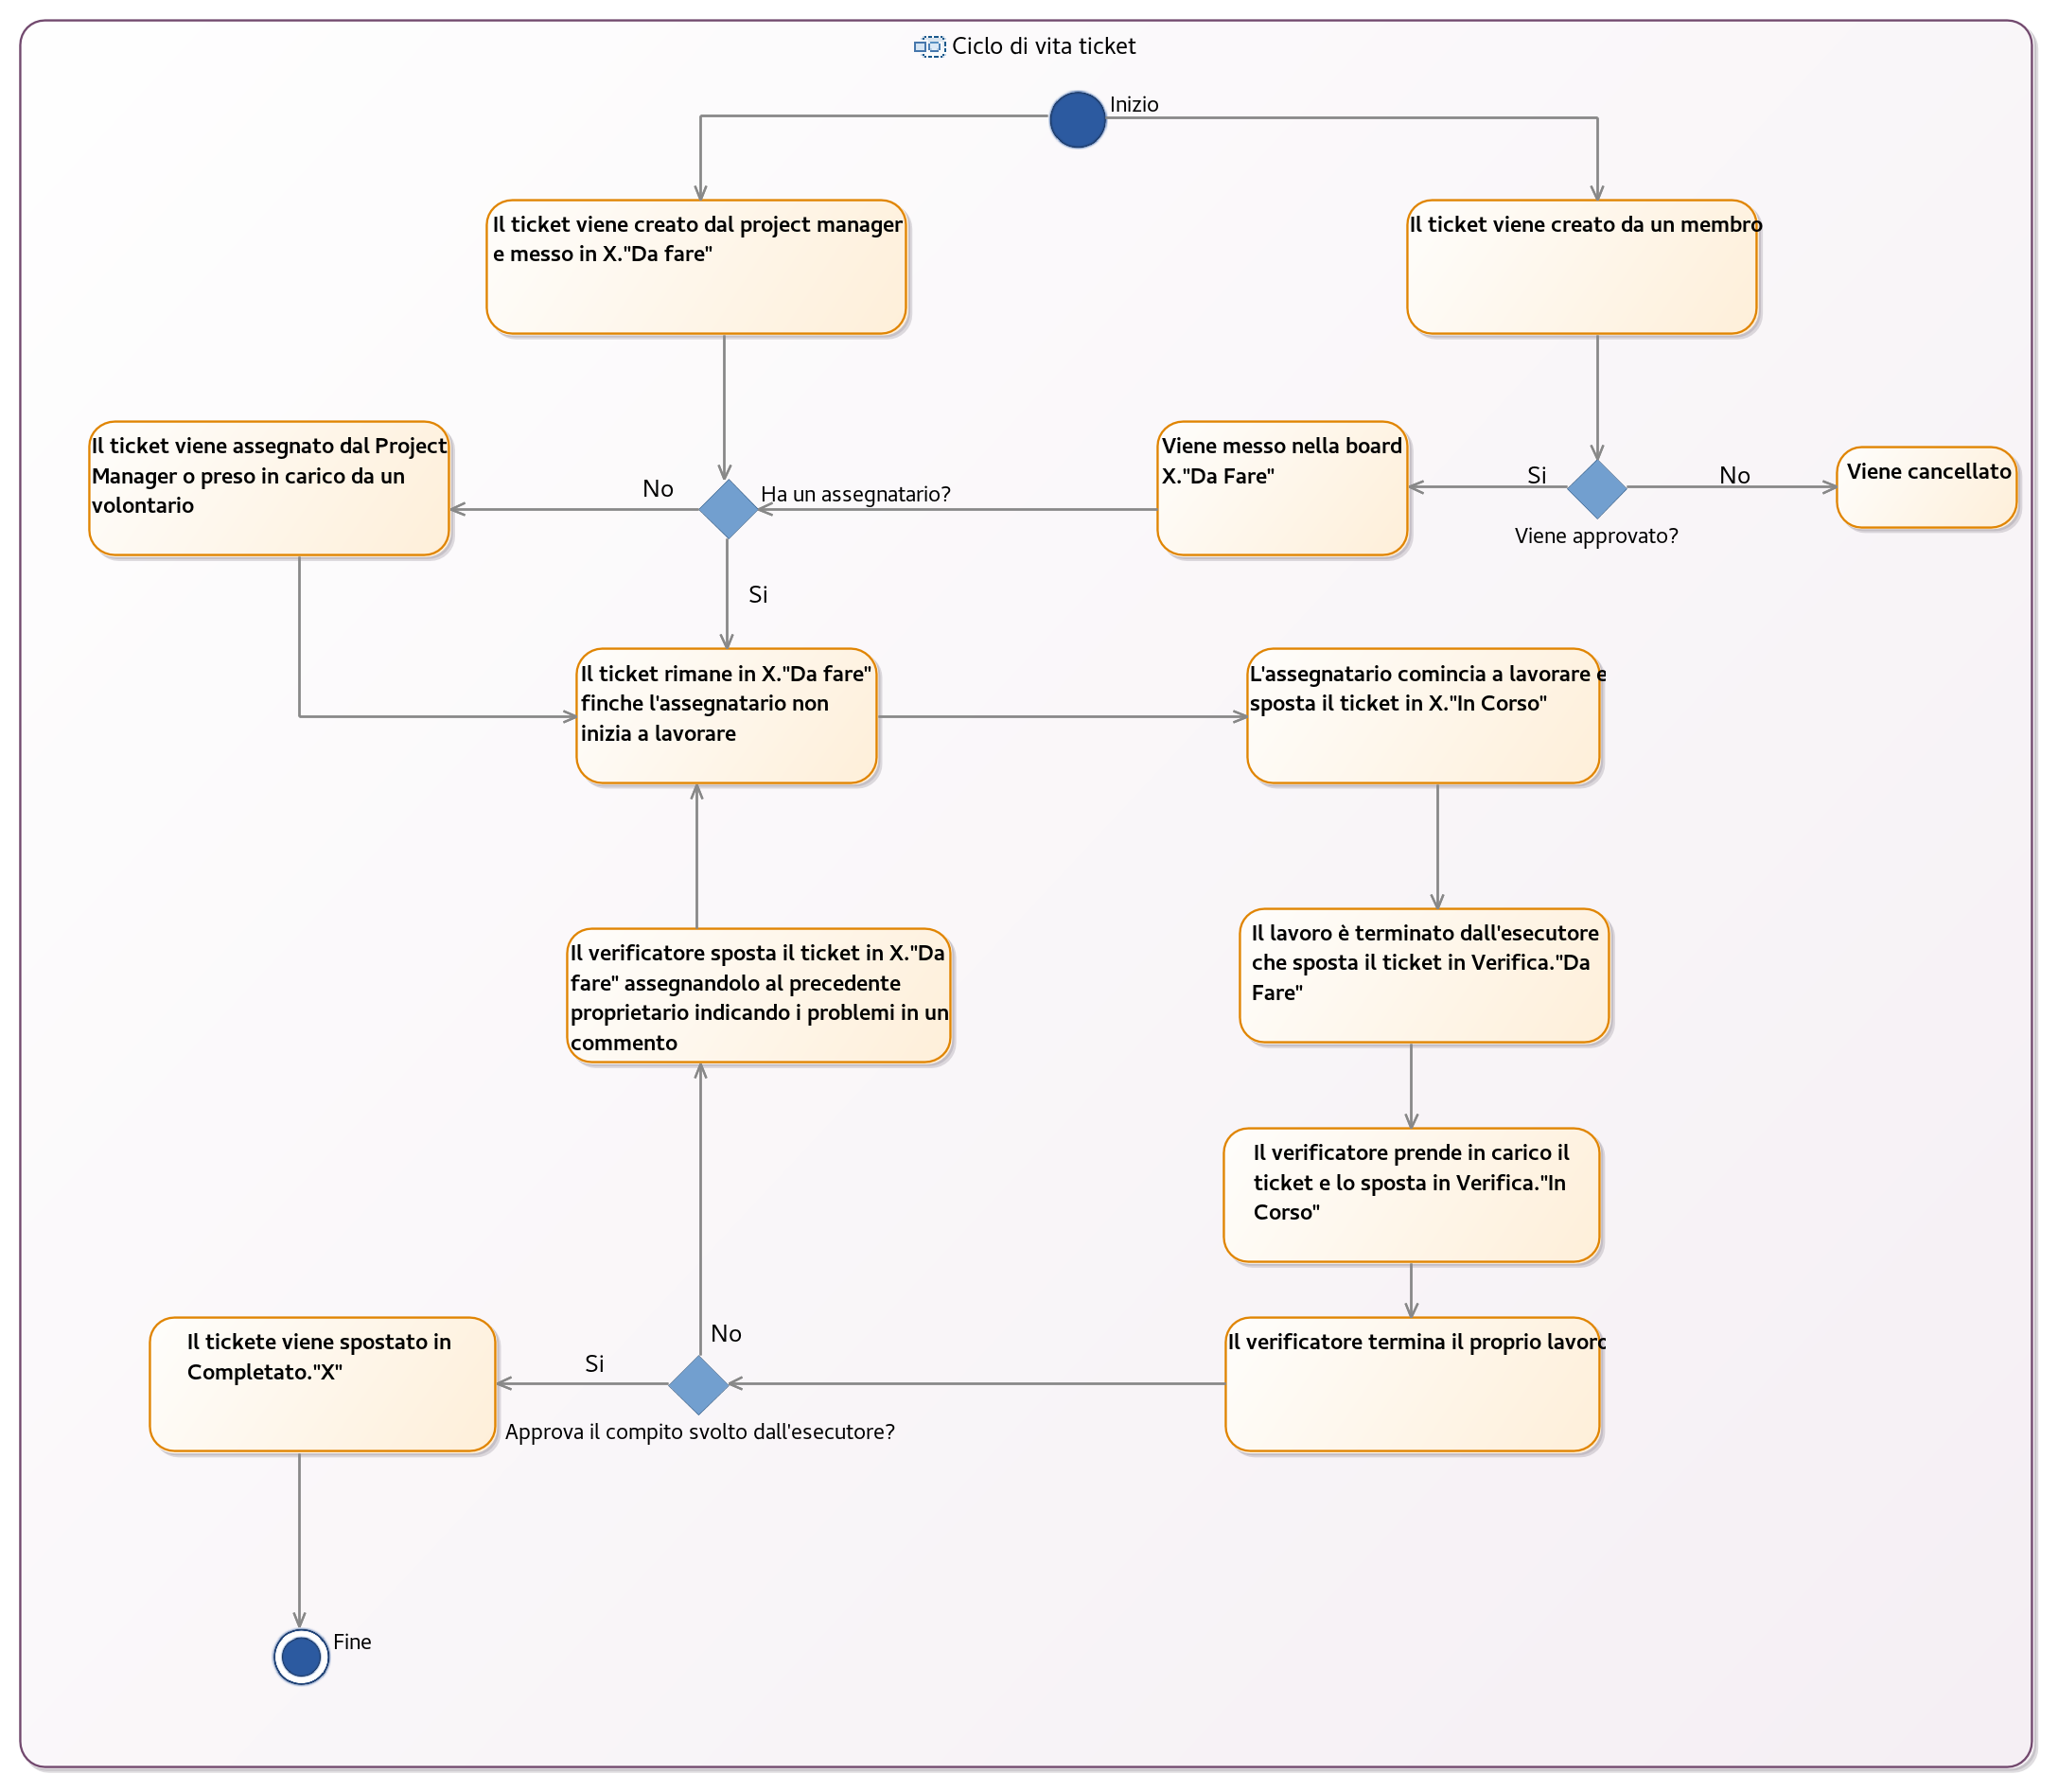
\includegraphics[scale=0.3]{../../common/images/AsanaFlow}
\end{document}